\documentclass[12pt, letterpaper]{article} 
 \usepackage{graphicx} 
 \usepackage{hyperref} 
 \usepackage[utf8]{inputenc} 
 \usepackage{float} 
 \usepackage{geometry} 
 \usepackage{enumitem, array} 
 \usepackage{longtable} 
 \usepackage{lscape} 
 \usepackage[export]{adjustbox} 
 \geometry{letterpaper,left=10mm,right=10mm,bottom=20mm,top=20mm} 
 \graphicspath{ {./../img/simulation/} } 
 \renewcommand{\rule}{Regla 22} 
 \renewcommand{\r}{22} 
 \title{ Reporte \rule } 
 \author{Fi App} 
 \begin{document} 
 \begin{titlepage} 
 \maketitle 
 \tableofcontents 
 \end{titlepage} 
 \clearpage 
 \begin{figure}[H]
  \centering
  \includegraphics[height=200mm,width=200mm,keepaspectratio]{simAnalysis.png} 
   \caption{Simulación de \rule} 
\end{figure}
\begin{table}[H]
  \centering
  \begin{tabular}{|c|c|c|c| }
     \hline Semilla-Densidad & Fill & Length & Steps  \\ 
      \hline    50 & 0 & 256 & 512 \\ 
      \hline 
       \end{tabular} 
      \caption{Datos de la simulación} 
    \end{table} 
\begin{section}{Análisis Fenotípico} 
  \begin{subsection}{Densidad} 
    \begin{figure}[H] 
      \centering 
       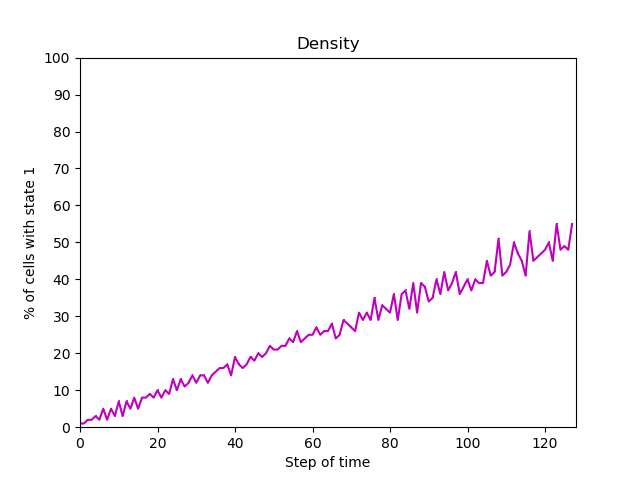
\includegraphics[max width=200mm ,max height=200mm , keepaspectratio ]{SimDensity.png} 
       \caption{Densidad de \rule} 
    \end{figure} 
  \end{subsection} 
  \begin{subsection}{Entropía} 
    \begin{figure}[H] 
    \centering 
    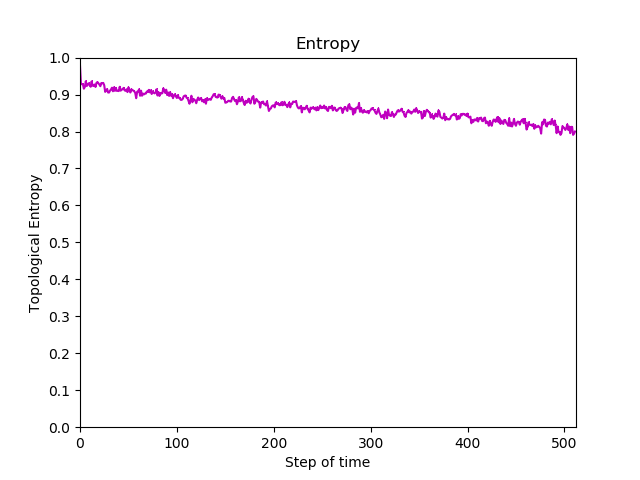
\includegraphics[max width=200mm ,max height=200 mm , keepaspectratio ]{SimEntropy.png} 
    \caption{Entropía de \rule} 
    \end{figure} 
    \end{subsection}
    \begin{subsection}{Exponentes de Lyapunov} 
    \begin{figure}[H] 
    \centering 
    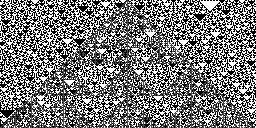
\includegraphics[max width=200mm ,max height=200 mm , keepaspectratio ]{SimDefects.png} 
    \caption{Simulación de los defectos del Exponentes de Lyapunov \rule} 
    \end{figure} 
    \end{subsection} 
    \begin{table}[H] 
    \centering 
    \begin{tabular}{cc} 
    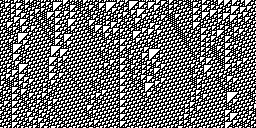
\includegraphics[width=70mm ,max height=70 mm , keepaspectratio]{SimAnalysis.png} & 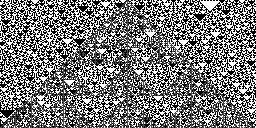
\includegraphics[width=70mm ,max height=70 mm , keepaspectratio]{SimDefects.png} \ 
    \end{tabular} 
    \caption{Simulación de la evolución original contra los defectos del Exponentes de Lyapunov \rule} 
    \end{table} 
    \begin{table}[H] 
    \centering 
    \begin{tabular}{cc} 
    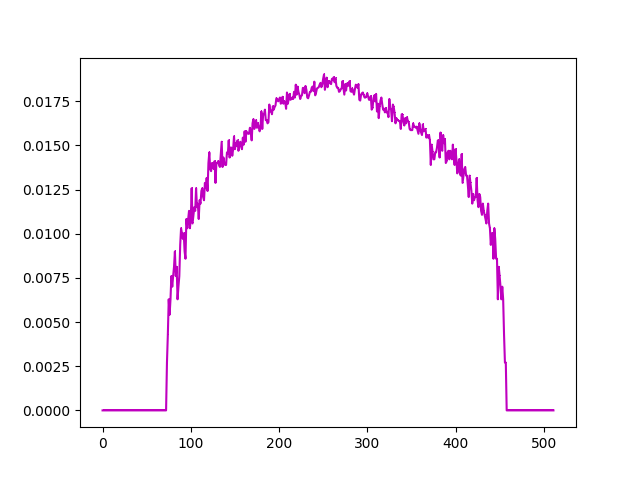
\includegraphics[width=90mm ,max height=90mm , keepaspectratio]{LyapunovExp.png} & 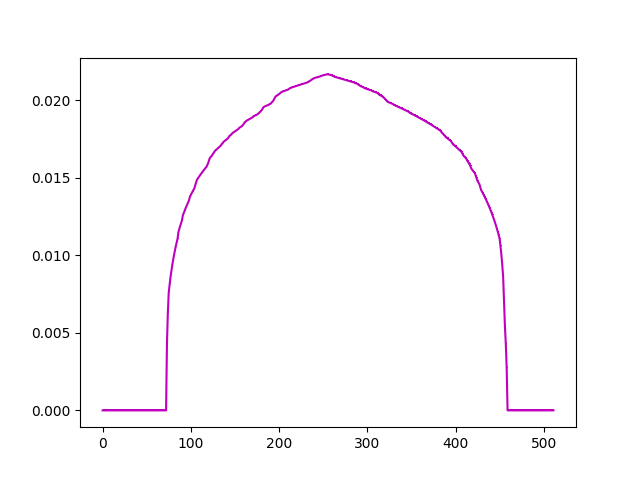
\includegraphics[width=90mm ,max height=90mm , keepaspectratio]{LyapunovExpNorm.png} \ 
    \end{tabular} 
    \caption{Simulación original contra los defectos del Exponentes de Lyapunov \rule} 
    \end{table} 
    \end{section} 
    \clearpage 
  \begin{section}{Análisis Genotípico} 
  \begin{subsection}{Teorìa del Campo Promedio}
  \begin{figure}[H]
  \centering
  \includegraphics[max width=200mm ,max height=200 mm , keepaspectratio ]{../img/MeanField/Plot\r.png}
  \caption{Gráfica del polinomio del campo promedio \rule  }
  \end{figure}
  \begin{table}[H]
  \centering
  \begin{tabular}{|c|c|c|c|}
  \hline Regla & Polinomio  & Punto fijo &Derivada \\ 
  \hline $\r$ & $3*(1 - x)^2*x$  &  $0.42265$  & $0.04639298528584379$ \\  \hline 
  \end{tabular}
  \caption{Datos de la gráfica del campo promedio}
  \end{table}
  \end{subsection}
  \clearpage
  \clearpage
  \begin{subsection}{Campos de atractores}
  \begin{center}
    \begin{longtable}{|c|c|c|c||c|c||c|}
  \hline 
  Num & Ciclo & Altura &Nodos &  Atractor &  Jardin del edén  & Entropia \\ \endhead 
